\chapter{Background}\label{ch:2}
Problems defined on networks arise in many real-life applications, such as finding the fastest route between two cities or computing the maximum bandwidth of an internet connection. A network can mathematically be represented by a graph. 

\newcommand{\Ein}[1]{\delta^-(#1)}
\newcommand{\Eout}[1]{\delta^+(#1)}
\newcommand{\ein}{{e_{\text{in}}}}
\newcommand{\eout}{{e_{\text{out}}}}

%for algorithms
%\newcommand{\setfont}[1]{\mathcal{#1}}
\newcommand{\setfont}[1]{#1}

%\section{math}
\begin{definition}[simple directed graph]
A graph is an ordered pair $G = (V, E)$ consisting of a vertex (or node) set $V$ and an edge (or arc) set $E$. The unqualified term "graph" usually refers to a \textit{simple} graph which has no multiple edges or self-loop edges. In a \textit{directed graph (digraph)}, $E$ is a set of ordered pairs of vertices, a subset of the cartesian product of vertices, that is $E \subseteq V \times V$. If the graph is simple, each edge $e \in E$ can be uniquely identified by a pair of vertices from $V$, that is $e=(v,w)$ with $v,w \in V$ and $v \neq w$, where $v$ is the start vertex and $w$ is the end vertex of the directed edge or arc $e$ \cite{jungnickel2013graphs}[1.6]. \end{definition}

\begin{figure}
\centering
	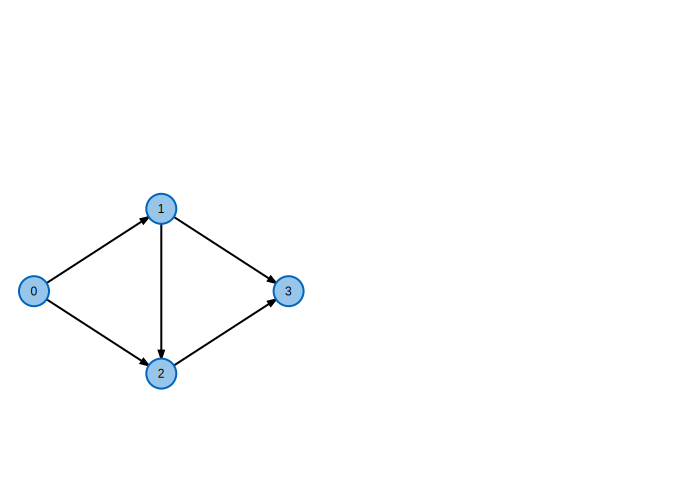
\includegraphics{fig/graph-editor}
	\caption{a digraph with $V=\{0,1,2,3\}$, $E=\{(0,1),(0,2),(1,2),(1,3),(2,3)\}$}
	\label{fig:graph}
\end{figure}

For problems and algorithms defined on digraphs, it is often convenient to define the set of edges coming into a vertex $v$ and zthe set of edges leaving it:
\begin{align}
\Ein{v}  &: \{ e=(u,v) \in E \; | \; u,v \in V \} \tag*{\eqnameformat{incoming edges}} \\
\Eout{v} &: \{ e=(v,w) \in E \; | \; v,w \in V \} \tag*{\eqnameformat{outgoing edges}}
\end{align}
In above example of a digraph \refFigure{fig:graph}, the vertex $v=2$ has an incoming edge set of $\Ein{2}=\{(0,2),(1,2)\}$ and an outgoing edge set of $\Eout{2}=\{(2,3)\}$.

\newpage
%\section{computer science}
Advanced algorithms to solve graph problems rely on common programming principles. The first one is so basic that it actually forms the basis of sorting algorithms such as \texttt{MergeSort}.
\begin{definition}[divide-and-conquer]
\textit{In divide-and-conquer, we solve a problem recursively, applying three steps at each level of the recursion:
\textbf{Divide} the problem into a number of subproblems that are smaller instances of the same problem. 
\textbf{Conquer} the subproblems by solving them recursively. If the subproblem sizes are small enough, however, just solve the subproblems in a straightforward manner. 
\textbf{Combine} the solutions to the subproblems into the solution for the original problem.} \cite[ch. 4]{cormen2009introduction}
\end{definition}

Recursion is clear and appealing from a mathematical perspective, but for computational efficiency reasons, divide-and-conquer is not always the best choice. It is better to remember useful intermediate results.
%\begin{definition}[recurrence]
%A recurrence relation is a mathematical formulation of the divide-and-conquer paradigm, an equation or inequality that descibes a function recursively in terms of base case and 
%\end{definition}

\begin{definition}[dynamic programming]
\textit{Dynamic programming, like the divide-and-conquer method, solves problems by combining the solutions to subproblems. %(“Programming” in this context refers to a tabular method, not to writing computer code.) 
[...] divide-and-conquer algorithms partition the problem into disjoint subproblems, solve the subproblems recursively, and then combine their solutions to solve the original problem. In contrast, dynamic programming applies when the subproblems overlap - that is, when subproblems share subsubproblems. In this context, a divide-and-conquer algorithm does more work than necessary, repeatedly solving the common subsubproblems. A dynamic-programming algorithm solves each subsubproblem just once and then saves its answer in a table, thereby avoiding the work of recomputing the answer every time it solves each subsubproblem.} \cite[ch. 15]{cormen2009introduction} 
%\cite[ch. 3, p. 70]{ahuja1993network}
\end{definition}
Dynamic programming can be applied to a wide range of graph problems, as we will see later. It works because of Bellman's:
\begin{definition}[Principle of Optimality]
\textit{An optimal policy has the property that whatever the initial state and initial decision are, the remaining decisions must constitute an optimal policy with regard to the state resulting from the first decision} \cite[sec. 3.3]{bellman1957dynamic}.
\end{definition}

For some kind of problems, we can get even more efficient with the greedy approach originating from matroid theory \cite[sec. 13.7, p. 528]{ahuja1993network} \cite[ch. 5]{jungnickel2013graphs}. It is at the heart of the efficient and well known Dijkstra algorithm.
\begin{definition}[greedy]
\textit{Algorithms for optimization problems typically go through a sequence of steps, with a set of choices at each step. For many optimization problems, using dynamic programming to determine the best choices is overkill; simpler, more efficient algorithms will do. A greedy algorithm always makes the choice that looks best at the moment. That is, it makes a locally optimal choice in the hope that this choice will lead to a globally optimal solution.} \cite[ch. 16]{cormen2009introduction}
\end{definition}
